\section*{Лекция №1: История вычислительной математики}
\addcontentsline{toc}{section}{Лекция №1}

\subsection*{Введение}
\addcontentsline{toc}{subsection}{Введение}

Развитие численных методов и становление науки вычислительной математики связано с необходимостью решения крупных научно- технических проблем и появлением быстродействующих электронно - вычислительных машин. С 1948 года  А. А. Самарский совместно с академиком А. Н. Тихоновым разрабатывал численные методы и вел первые в СССР прямые расчеты мощности взрыва атомной, а позже — водородной бомбы, необходимые для проведения дальнейших экспериментов. В этих работах были заложены основы математического моделирования и созданы важнейшие принципы конструирования и обоснования разностных схем и параллельных вычислений. 

Успехи ядерной физики, и в первую очередь, создание атомной бомбы, атомной энергетики, искусственных спутников Земли потребовали развития и широкого применения методов математического моделирования, а вместе с этим, развития вычислительной техники и подготовки специалистов-математиков, использующих эту технику.

\subsection*{Разностная аппроксимация простейших дифференциальных операторов}
\addcontentsline{toc}{subsection}{Разностная аппроксимация}

\subsubsection*{Сетки и сеточные функции}
\addcontentsline{toc}{subsubsection}{Сетки и сеточные функции}

Для того чтобы написать разностную схему, приближенно описывающую данное дифференциальное уравнение, нужно совершить следующие два шага.

\begin{enumerate}
	\item Необходимо заменить область непрерывного изменения аргумента областью дискретного его изменения.
	\item Необходимо заменить дифференциальный оператор некоторым разностным оператором, а также сформулировать разностный аналог для краевых условий и для начальных данных.
\end{enumerate}

После осуществления такой процедуры мы приходим к алгебраической системе уравнений. Таким образом, задача о численном решении исходного (линейного) дифференциального уравнения сводится к вопросу о нахождении решения полученной алгебраической системы.

Остановимся на этих вопросах несколько подробнее.

При численном решении той или иной математической задачи мы, очевидно, нө можем воспроизвести разностное решение для всех значений аргумента, изменяющегося внутри некоторой области евклидова пространства.

Естественно поэтому выбрать в этой области некоторое конечное множество точек и приближенное решение искать только в этих точках. Такое множество точек называется сеткой. Отдельные точки называют узлами сетки.

Функция, определенная в узлах сетки, называется сеточной функцией. Таким образом, мы заменили область непрерывного изменения аргумента сеткой, т. е. областью дискретного изменения аргумента; иными словами, мы осуществили аппроксимацию пространства решений дифференциального уравнения пространством сеточных функций.

Свойства разностного решения и, в частности, его близость к точному решению зависят от выбора сетки.

\textbf{Пример 1}. Равномерная сетка на отрезке. Разобьем единичный отрезок $[0,1]$ на $N$ равных частей. Расстояние между соседними узлами $x_i-x_{i-1}=h=1 / N$ назовем шагом сетки. Точки деления $x_i=i h-$ узлы сетки. Множество всех узлов $\omega_h=\left\{x_i=\right.$ $=i h, i=1,2, \ldots, N-1\}$ и составляет сетку (рис. 1), в данном случае введенную на отрезке.

\begin{wrapfigure}{r}{0.5\textwidth}
	\centering
	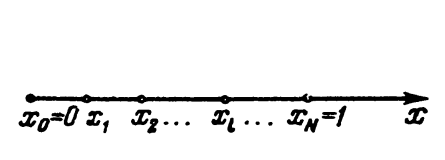
\includegraphics[width=0.5\textwidth]{img/1.png}
	\caption{}
	\label{fig:1}
\end{wrapfigure}


В это множество можно включить граничные - точки $x_0=0, \quad x_N=1$. Обозначим $\bar{\omega}_h=\left\{x_i=i h, i=0,1, \ldots\right.$ ..., $N-1, N\}$.
(рис.~\ref{fig:1}) 
На отрезке [0,1] вместо функции непрерывного аргумента $y(x)$ будем рассматривать функцию дискретного аргумента $y_h\left(x_i\right)$. Значения этой функции вычисляются в узлах сетки $x_i$, а сама функция зависит от шага сетки $h$ как от параметра.

\textbf{Пример 2}. Равномерная сетка на плоскости. Рассмотрим множество функций двух аргументов $u(x, t)$. В качестве области определения выберем прямоугольник

$$
\overline{D}=\{0 \leqslant x \leqslant 1, \quad 0 \leqslant t \leqslant T\} .
$$

\begin{wrapfigure}{r}{0.5\textwidth}
	\centering
	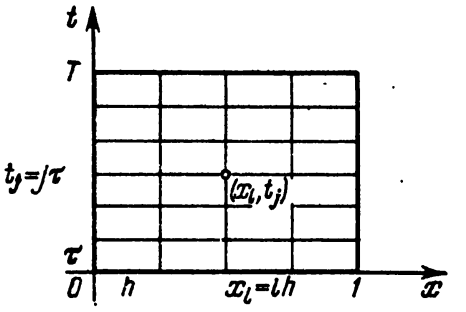
\includegraphics[width=0.5\textwidth]{img/2.png}
	\caption{}
	\label{fig:2}
\end{wrapfigure}


Разобьем отрезки $[0,1]$ оси $x$ и $[0, T]$ оси $t$ соответственно на. $N_1$ и $N_2$ частей; пусть $h=1 / N_1$, $\tau=T / N_2$. Через точки деления проведем прямые, параллельные соответствующим осям. В результате пересечения этих прямых получим узлы ( $\left.x_i, t_j\right)$, которые и образуют сетку (рис.~\ref{fig:2}) 

$$
\overline{\omega_{h \tau}}=\left\{\left(x_i, t_j\right) \in \overline{D}\right\} .
$$

Эта сетка имеет шаги $h$ и $\tau$ соответственно по направлениям $x$ и $t$. Соседними узлами сетки называются узлы, лежащие на одной и той же прямой (горизонтальной или вертикальной), расстояние между которыми равно шагу сетки ( $h$ или $\tau$ ).

\textbf{Пример 3}. Неравномерная сетка на отрезке. Рассмотрим отрезок $0 \leqslant x \leqslant 1$. Вводя произвольные точки $0<x_1<x_2<\ldots$... $\ldots<x_{N-1}<1$, разобьем его на $N$ частей. Множество узлов $$\left\{x_i : i=0, \ldots, N, \quad x_0=0, x_N=1\right\}$$ образует неравномерную сетку $\widehat{\omega}_h[0,1]$. Расстояние между соседними узлами - шаг сетки - равно $h_i=x_i-x_{i-1}$ п зависит уже от номера $i$ узла, т. е. является сеточной функцией. Шаги сетки удовлетворяют условию нормировки

$$
\sum_{i=1}^N h_i=1
$$

\textbf{Пример 4}. Сетка в двумерной области. Пусть на плоскости $x=\left(x_1, x_2\right)$ дана область $G$ сложной формы с границей $\Gamma$. Проведем прямые $x_1^{\left(i_1\right)}=i_1 h_1, i_1=0, \pm 1, \pm 2, \ldots, h_1>0 ; x_2^{\left(i_2\right)}=i_2 h_2, i_2=$ $=0, \pm 1, \pm 2, \ldots, h_2>0$. Тогда на плоскости ( $x_1, x_2$ ) получим сетку (решетку) с узлами ( $\left.i_1 h_1, i_2 h_2\right), i_1, i_2=0, \pm 1, \pm 2, \ldots$

\begin{wrapfigure}{l}{0.45\textwidth}
	\centering
	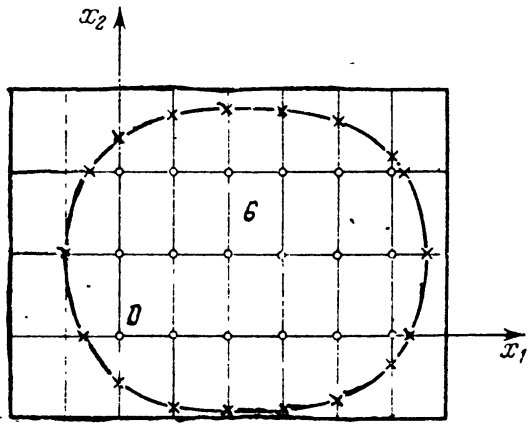
\includegraphics[width=0.45\textwidth]{img/3.png}
	\caption{}
	\label{fig:3}
\end{wrapfigure}

Эта решетка равномерна по каждому из направлений $O x_1$ и $O x_2$. Нас интересуют только те узлы, которые принадлежат области $\bar{G}=G+\Gamma$, включая границу $\Gamma$. Те узлы ( $i_1 h_1, i_2 h_2$ ), которые попали внутрь $G$, назовем внутренними, а их совокупность обозначим $\omega_h$ (рис. 3). Рассмотрим точки пересечения прямых $x_1^{\left(i_1\right)}=i_1 h_1 \quad$ и $\quad x_2^{\left(i_2\right)}=i_2 h_2$, $i_1, i_2=0, \pm 1, \pm 2, \ldots$, с границей $\Gamma$; эти точки назовем граничными узлами, а множество всех граничных узлов обозначим $\gamma_h$. На (рис.~\ref{fig:3})  знаком $\times$ обозначены граничные узлы, а значком - - внутренние узлы. Из (рис.~\ref{fig:3})  видно, что имеются граничные узлы, которые отстоят от ближайших к ним внутренних узлов на расстоянии, меньшем $h_1$ или $h_2$. Таким образом, хотя сетка на плоскости и равномерна по $x_1$ и $x_2$, но сетка $\bar{\omega}_h=\omega_h+\gamma_h$ для области $\bar{G}$ неравномерна вблизи границы.

Итак, область $\bar{G}$ изменения аргумента $x$ мы заменяем сеткой $\bar{\omega}_h$, т. е. конечным множеством точек $x_i$, принадлежащих $\bar{G}$. Вместо функций $u(x)$ непрерывного аргумента $x \in \bar{G}$ будем рассматривать сеточные функции $y\left(x_i\right)$, т. е. функции точки $x_i$, являющейся узлом сетки $\bar{\omega}_h=\left\{x_i\right\}$. Сеточную функцию $y\left(x_i\right)$ можно представить в виде вектора. Если перенумеровать все узлы в некотором порядке $x_1, x_2, \ldots, x_N$, то значения сеточной функции в этих узлах можно рассматривать как компоненты вектора

$$
Y=\left(y_1, \ldots, y_i, \ldots, y_N\right) .
$$

Если область $G$, в которой построена сетка, конечна, то размерность $N$ вектора $Y$ конечна. В случае неограниченной области $G$ сетка состоит из бесконечного числа узлов и размерность вектора $Y$ также бесконечна.

Обычно рассматриваются множества сеток $\left\{\omega_h\right\}$, зависящих от шага $h$ как от параметра. Поэтому и сеточные функции $y_h(x)$ зависят от параметра $h$ (или от числа узлов $N$ в случае равномерной сетки). Если сетка $\omega_h$ неравномерна, то под $h$ следует понимать вектор $h=\left(h_1, h_2, \ldots, h_N\right)$ с компонентами $h_1, \ldots, h_N$.
